\section{Problemstellung und Ansatz}




Softwaretests sind ein wichtiger Baustein für die Qualitätssicherung von Softwareprojekten. Für Tests von Datenbank-basierten Anwendungen müssen u.a.~Testdaten für die Datenbank spezifiziert werden, auf deren Basis das Verhalten der zu testenden Software 
%(System Under Test, SUT) 
geprüft werden kann.
%
%
Die Spezifikation dieser Testdaten ist leider augenblicklich sehr umfangreich und komplex und somit aufwändig und fehleranfällig.
%
%Bei datenbank-basierten Anwendungen sind die Testdaten meist sehr umfangreich und komplex.
%
Die Komplexität ergibt sich v.a.~aus der Beschreibung der Beziehungen zwischen den einzelnen Entitäten.
%im Test Fixture.
%
Diese unterliegen einer Menge komplexer fachlicher Regeln, die sich aus dem Domänen-Modell und der Geschäftslogik der Anwendung ergeben.
%
%%%Besonders bei Systemen mit großen oder komplexen Datenbank-Schemata kann ein Testdaten-Set schnell unübersichtlich werden.


Übergreifendes Ziel der hier beschriebenen Arbeit \cite{MT:Moll:2013} war es, die Spezifikation von Testdaten für Datenbank-basierte Java-Anwendungen zu vereinfachen.
%
Hierzu wurde zum einen  eine geeignete Domänen-spezifische Sprache (DSL) für Testdaten entwickelt.
%
%%%Die DSL erlaubt eine  übersichtliche Spezifikation von Testdaten, ist einfach zu nutzen und integriert sich in gängige Entwicklungsumgebungen.
%
Zum anderen wurde ein Generator zur automatischen Erzeugung von Testdaten implementiert. 
%
%%%Das Ziel hierbei war es, mit möglichst wenig Datensätzen viele Grenzfälle bei Beziehungen abzudecken.
%
%
Basis der Entwicklungsarbeiten war die Java-Bibliothek Simple Test Utils for JUnit \& Co. (STU) zur Vereinfachung von Unit-Tests für Java-Anwendungen.
%
STU steht unter der Apache License 2.0 und wird federführend von der  SEITENBAU GmbH entwickelt. 
%
%%%Für Tests von Datenbank-basierten Anwendungen setzt STU auf der Bibliothek DbUnit auf.


\begin{figure}[tb]
	\begin{center}
		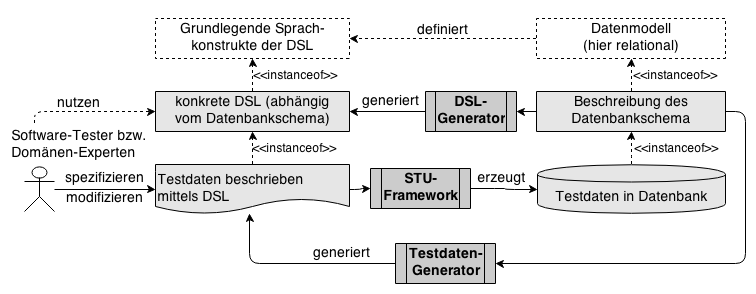
\includegraphics[width=12.75cm]{images/ansatz.png}
		\caption{\label{ansatz}Überblick über den gewählten Ansatz.}
	\end{center}
   %\vspace{-0.5cm}  %%% BAD HACK JW
\end{figure}

Abb.~\ref{ansatz} gibt einen Überblick über den gewählten, modellgetriebenen Ansatz.
%
Ausgangspunkt ist eine formale Beschreibung des relationalen Datenbankschemas (Details siehe \cite{MT:Moll:2013}).
%
Diese kann mittels eines Tools (nicht dargestellt) manuell erstellt bzw.~aus einer existierenden Datenbank extrahiert und ergänzt werden.
%
Aus der Schema-Beschreib\-ung wird die Schema-abhängige Testdaten-DSL generiert. 
%
Diese DSL kann dann von den Testern genutzt werden, um verschiedene Testdaten-Sets zu beschreiben und diese mittels STU in ihre Unit-Tests einzubinden.
%
Die Testdaten-Sets werden bei den Tests durch das STU-Framework automatisch in die Datenbank eingespielt.
%
%%%(Backdoor-Manipulation \cite{XUNIT_TEST_PATTERNS}). 
%
Auf Basis der Schema-Be\-schrei\-bung können auch in der DSL beschriebene Test\-da\-ten-Sets  generiert werden. Die generierten Testdaten können ggfls.~vor Verwendung noch angepasst werden.
%
%
%
%Details und ausführliche Code-Beispiele zur Verwendung sind in \cite{MT:Moll:2013} zu finden.





	




